\section{Modelli computazionali}

In questo lavoro sono state utilizzate tecnologie con differenti modelli computazionali che
hanno portato a differenti soluzioni tecniche per effettuare una coerente integrazione dei sistemi utilizzati.
\marianiSays{ingrandirei anche la 2.3}
\subsection{Unity event loop}

Il modello computazionale presente su Unity è event loop: questo significa che tutti gli elementi presenti nella scena, come Script e GameObject, sono vincolati ad uno specifico lifecycle (raffigurato nell'immagine sottostante).
\begin{figure}[H]
   \centering
   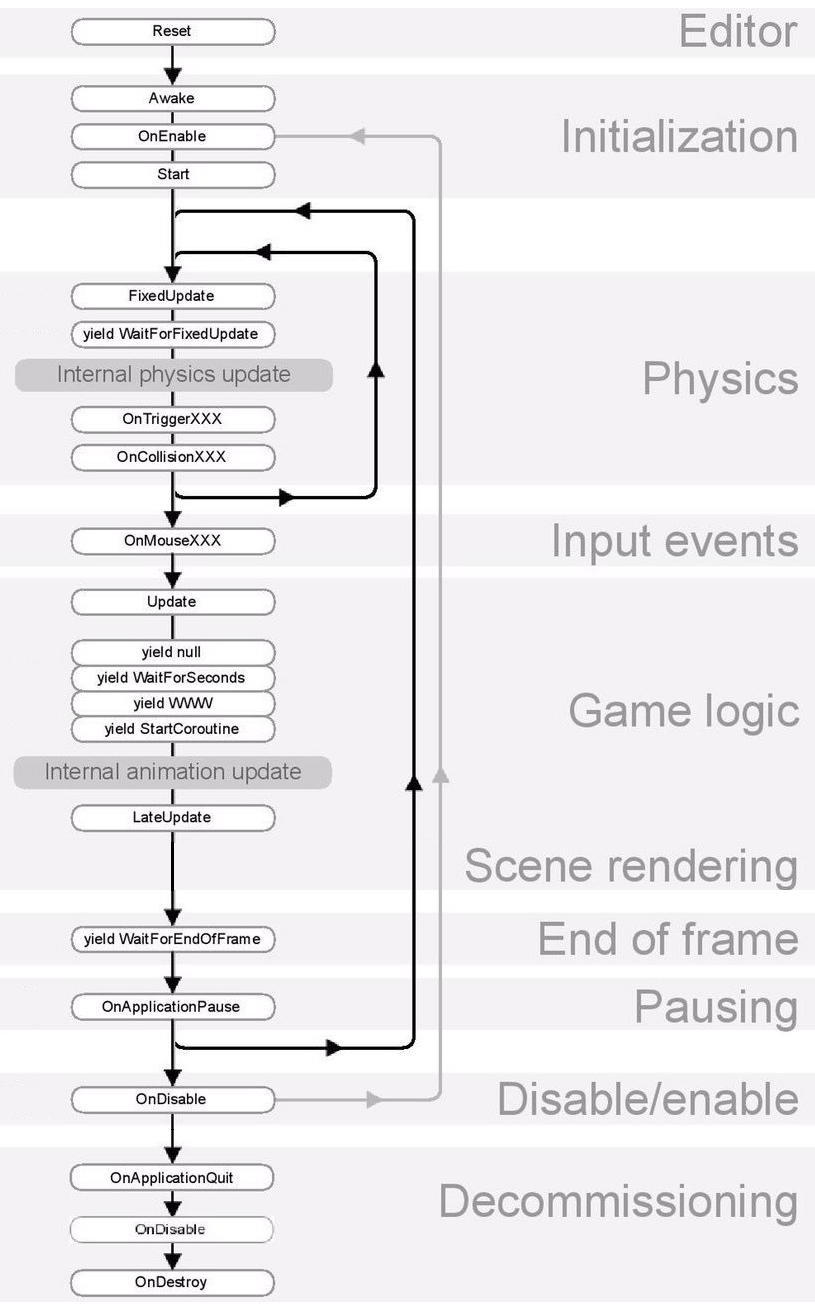
\includegraphics[height=\linewidth]{figures/Unity_lifecycle.jpeg}
   \caption{Unity lifecycle\cite{unity}}
\end{figure}

\improvement[inline]{Spiegare come ho fatto per notificare le "azioni" ai corpi}

Per interagire internamente tra i componenti, Unity mette disposizione delle API definite come "Event System"
con le quali è possibile inviare eventi agli oggetti nell'applicazione in base all'input, che si tratti di tastiera, mouse, tocco o input personalizzato.

Link utili:
\begin{itemize}
   \item \href{https://docs.unity3d.com/2018.3/Documentation/Manual/MessagingSystem.html}{Unity Messaging System}
   \item \href{https://docs.unity3d.com/2018.3/Documentation/Manual/MessagingSystem.html}{Unity Messaging System}: Utilizzato per generare eventi di ricezione nuovi messaggi direttamente inviati dalla WebSocket al VirtualBody invece di lasciare il VirtualBody a fare polling sulla coda dei messaggi in ingresso)
\end{itemize}

\subsection{Modello ad attori in Play}

\subsection{Jason BDI}

\subsection{CArtAgO}
